\documentclass[border=8pt]{standalone}
\usepackage{amsmath,amssymb,bm}
\usepackage{xcolor}
\usepackage{tikz}
\definecolor{P}{HTML}{4B1D8F}
\definecolor{ink}{HTML}{1B1B2F}
\colorlet{band}{P!7!white}
\colorlet{lcol}{P!14!white}
\colorlet{rule}{P!45!white}
\begin{document}
\Large
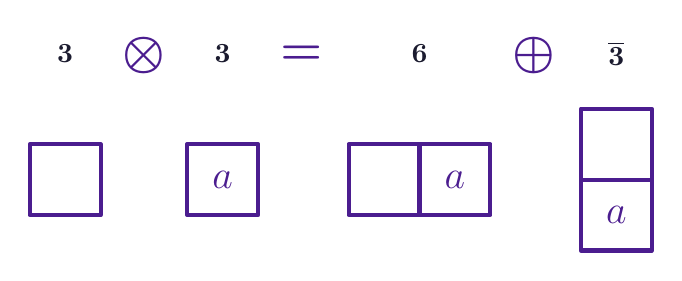
\begin{tikzpicture}[every node/.style={text=ink}]
\node at (0.000,0) {$\mathbf{3}$};
\draw[P,line width=1.5pt,line join=round,rounded corners=0pt] (-0.450,-1.150) rectangle (0.450,-2.050);
\node[text=P] at (1.000,-.02) {\LARGE$\bm{\otimes}$};
\node at (2.000,0) {$\mathbf{3}$};
\draw[P,line width=1.5pt,line join=round,rounded corners=0pt] (1.550,-1.150) rectangle (2.450,-2.050);
\node[text=P] at (2.000,-1.600) {\Large$a$};
\node[text=P] at (3.000,-.02) {\LARGE$\bm{=}$};
\node at (4.500,0) {$\mathbf{6}$};
\draw[P,line width=1.5pt,line join=round,rounded corners=0pt] (3.600,-1.150) rectangle (5.400,-2.050);
\draw[P,line width=1.5pt] (4.500,-1.150) -- (4.500,-2.050);
\node[text=P] at (4.950,-1.600) {\Large$a$};
\node[text=P] at (5.950,-.02) {\LARGE$\bm{\oplus}$};
\node at (7.000,0) {$\overline{\mathbf{3}}$};
\draw[P,line width=1.5pt,line join=round,rounded corners=0pt] (6.550,-0.700) rectangle (7.450,-2.500);
\draw[P,line width=1.5pt] (6.550,-1.600) -- (7.450,-1.600);
\node[text=P] at (7.000,-2.050) {\Large$a$};
\end{tikzpicture}
\end{document}
